\section{Preliminaries}
\label{sec:background}

\subsection{Networks of Timed Automata}

The timed automaton model used in this paper follows the standard timed-automata
semantics~\cite{bengtsson2004timed}.

\noindent\textbf{Definition 1.}
A timed automaton (TA) is a tuple
\begin{equation}
  T=(L,\ell_0,C,\Sigma,\Theta,I)
\end{equation}
where $L$ is a finite set of locations, $\ell_0$ is the initial location,
$C$ is a finite set of clocks, $\Sigma$ is a set of action labels,
$\Theta$ is a finite set of transitions, and $I$ maps each location to a
clock invariant. A clock constraint is a conjunction of atoms $x\sim b$,
where $x\in C$, $\sim\in\{<,\leq,=,\geq,>\}$, and
$b\in\mathbb{R}_{\geq 0}$. A transition
$\theta=(\ell,g,a,R,\ell')$ moves from $\ell$ to $\ell'$ when guard $g$
is satisfied, emits action $a$, and resets clocks in $R\subseteq C$.
An NTA is a parallel composition
$\mathcal{N}=T_1\parallel\cdots\parallel T_k$ with the synchronization
semantics of the target modeling language, such as UPPAAL
\cite{larsen1997uppaal}. Its behavior consists of action and delay
transitions. Action transitions are instantaneous, require their guards
to be satisfied, and reset the specified clocks; delay transitions model
the passage of time in a location while respecting its invariant.

\subsection{Timed Diagnostic Traces (TDTs) and Multi-Property Motivation}

This paper focuses on timed safety properties, which are commonly used
to specify deadlines, bounded waiting, and reachable error states in
real-time systems. Such properties can be checked by tools such as
UPPAAL: given an NTA and a property, the verifier either confirms the
property or returns a counterexample trace~\cite{vogel2022patterns}.

\noindent\textbf{Definition 2.}
A symbolic timed trace (STT) of a model is a finite transition sequence
$S=\theta_0,\ldots,\theta_{n-1}$. A realization of $S$ is a sequence of
non-negative delays $d_0,\ldots,d_n$ and states
$s_0,\ldots,s_{n+1}$ such that, for every $i<n$, the model can delay
from $s_i$ by $d_i$ and then take $\theta_i$ to $s_{i+1}$ while
respecting guards, resets, invariants, and synchronizations; the final
delay $d_n$ leads from $s_n$ to $s_{n+1}$. The STT is feasible if it has
at least one realization. Given a safety property $\varphi$, a feasible
STT is a TDT for $\varphi$ if at least one realization reaches a state
that violates $\varphi$.

\begin{figure}[t]
  \centering
  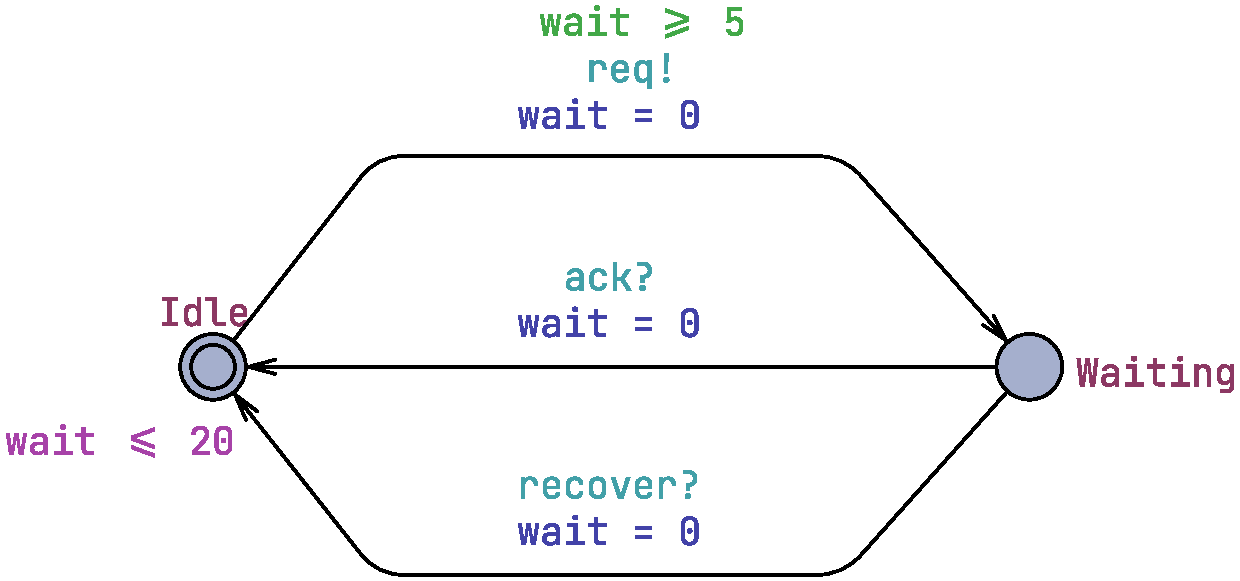
\includegraphics[width=0.58\columnwidth]{figures/gear_shift_nta_Driver-cropped.pdf}\\[-0.35em]
  {\footnotesize (a) Driver}\\[0.2em]
  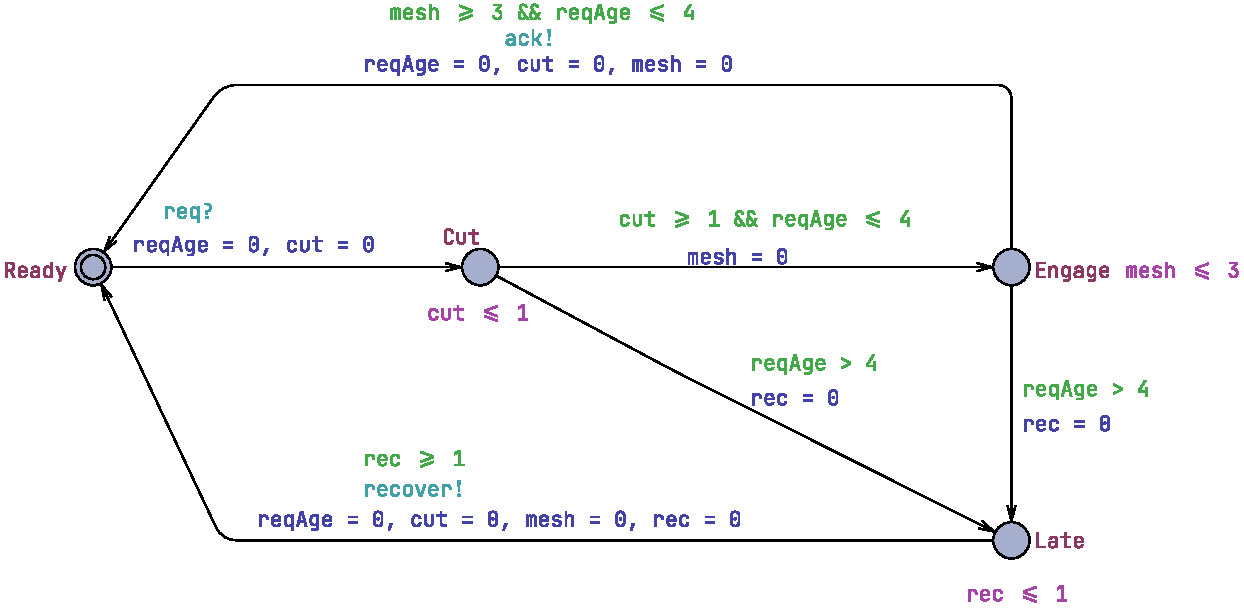
\includegraphics[width=0.98\columnwidth]{figures/gear_shift_nta_GearController-cropped.pdf}\\[-0.55em]
  {\footnotesize (b) GearController}
  \caption{Simplified gear-shift example.}
  \label{fig:gear-shift-nta}
  \vspace{-0.5em}
\end{figure}

\noindent\textit{Example 1.}
Figure~\ref{fig:gear-shift-nta} shows the running gear-shift example.
The Driver issues a request through $\mathit{req}!$, and the controller
responds through $\mathit{ack}!$ or $\mathit{recover}!$. In the faulty
controller, $\mathit{cut}\leq 1$ and $\mathit{cut}\geq 1$ allow
engagement after one time unit, violating property $\varphi_1$, which
requires at least two time units of torque cut. A single-property repair
can change these bounds to $2$. However, if the
$\mathit{mesh}\leq 3$ and $\mathit{mesh}\geq 3$ bounds remain unchanged,
the earliest acknowledgement occurs after $2+3=5$ time units, violating
property $\varphi_2$, which requires acknowledgement within four time
units. A multi-property repair must therefore adjust both
$\mathit{cut}$ and $\mathit{mesh}$ while preserving the original
functional behavior, including the request--engage--acknowledge path.

TDTs provide concrete realizations of property violations, but they do
not explain why the violations occur. In particular, a TDT does not
identify which numerical bound is faulty or whether the relevant bound
appears in a guard or an invariant. Following the idea of TARTAR
\cite{kolbl2019clock}, the repair procedure developed later in this
paper encodes TDTs as arithmetic constraints over trace feasibility,
property violation, and bound variations. Unlike single-property repair,
MPTA-Repair organizes constraints from multiple violated properties and
TDTs into a joint solving process to generate candidate clock-bound
repairs.

Let $M_{\mathit{bad}}$ be a faulty NTA model and let
$\Phi=\{\varphi_1,\ldots,\varphi_m\}$ be the set of properties that must
be satisfied simultaneously. MPTA-Repair generates a repaired model
$M_{\mathit{rep}}$ by changing repairable numerical bound occurrences
in guards and invariants. A candidate repair is accepted only if
\begin{equation}
  M_{\mathit{rep}}\models \bigwedge_{\varphi\in\Phi}\varphi
  \quad\land\quad
  \mathrm{Accept}(M_{\mathit{bad}},M_{\mathit{rep}}).
\end{equation}
The first condition requires the repaired model to satisfy all required
properties. The second condition denotes a TARTAR-style admissibility
check based on functional equivalence~\cite{kolbl2019clock}. This check
prevents repairs that satisfy properties merely by disabling required
actions.
